% Движок: LuaLaTeX (Menu -> Compiler -> LuaLaTeX). Компилировать дважды.
% Схемы из части I подключаются как готовые PDF из figs/ — исходники TikZ
% лежат в figs_src/ (см. README).
\documentclass[aspectratio=169,10pt]{beamer}
\usepackage[T2A,T1]{fontenc}
\usepackage[utf8]{inputenc}
\usepackage[english,russian]{babel}
\usepackage{lmodern}
\usepackage{textcomp}
\usepackage{graphicx}
\graphicspath{{figs/}}

\usepackage{booktabs}
\usepackage{array}

\usetheme{default}
\usecolortheme{default}
\setbeamertemplate{navigation symbols}{}
\setbeamercolor{frametitle}{fg=black}
\setbeamerfont{frametitle}{size=\large,series=\bfseries,family=\sffamily}
\setbeamertemplate{footline}{%
  \hfill\scriptsize\color{gray!70!black}\insertframenumber\;/\;\inserttotalframenumber\hspace{3ex}\vspace{3.5ex}}

\definecolor{cProved}{HTML}{1B6B3A}
\definecolor{cFound}{HTML}{9A5B00}
\definecolor{cTrivial}{HTML}{3A5A8C}
\definecolor{cInk}{HTML}{1A1A1A}
\definecolor{cMuted}{HTML}{6B6B6B}
\definecolor{cLine}{HTML}{BFBFBF}
\definecolor{cLayA}{HTML}{7E9DC4}
\definecolor{cLayB}{HTML}{DE9A4E}
\definecolor{cLayC}{HTML}{6FB07F}

\newcommand{\statusProved}{\textcolor{cProved}{\textbf{Оптимальность доказана}}}
\newcommand{\statusFound}{\textcolor{cFound}{\textbf{Лучшая известная конструкция}}}
\newcommand{\statusTrivial}{\textcolor{cTrivial}{\textbf{Тривиальная упаковка}}}
\newcommand{\statusTrivBest}{\textcolor{cTrivial}{\textbf{Тривиальная — лучшая известная}}}

% --- Картинки или плейсхолдеры ----------------------------------------------
% Плейсхолдеры включены по умолчанию. Чтобы подставить настоящие картинки,
% положите файлы 1.png, 2.png, ... в папку figs/ и переключите флаг ниже
% (false -> true).
\newif\ifuseimages
\useimagestrue

% Рамка-плейсхолдер (без TikZ, чтобы сборка была быстрой)
% #1 - сторона в см, #2 - имя файла, #3 - толщина рамки в pt
\newcommand{\imgphbox}[3]{%
  \begingroup
  \setlength{\fboxsep}{0pt}\setlength{\fboxrule}{#3pt}%
  \fcolorbox{cLine}{gray!6}{%
    \begin{minipage}[c][#1cm][c]{#1cm}%
      \centering\color{cMuted}\sffamily\tiny\texttt{#2}%
    \end{minipage}}%
  \endgroup}

% Большой кадр: #1 - сторона в см, #2 - имя файла в figs/
\newcommand{\imgph}[2]{%
  \ifuseimages\includegraphics[width=#1cm,height=#1cm,keepaspectratio]{#2}%
  \else\imgphbox{#1}{#2}{0.9}\fi}

% Компактный кадр для сетки 2x2
\newcommand{\imgphs}[2]{%
  \ifuseimages\includegraphics[width=#1cm,height=#1cm,keepaspectratio]{#2}%
  \else\imgphbox{#1}{$n=#2$}{0.8}\fi}

\title{Задачи об упаковке}
\subtitle{Часть I: плотнейшая упаковка шаров \quad\textbullet\quad Часть II: единичные квадраты в квадрате}
\author{Часть I: схемы построены средствами TikZ\\ Часть II: данные и схемы упаковок — Erich Friedman, \emph{Squares in Squares}}
\date{}

\begin{document}

\begin{frame}[plain]
  \titlepage
  \vspace{-1em}
  \begin{center}\footnotesize\color{cMuted}
  Часть II, источник данных: \texttt{https://tabatkins.github.io/efmath/packing/squinsqu/}
  \end{center}
\end{frame}

\begin{frame}[plain]
\vfill
\centering
{\Large\bfseries Часть I. Плотнейшая упаковка одинаковых шаров}\\[6pt]
{\color{cMuted}\small гипотеза Кеплера, слои $A$, $B$, $C$ и кристаллические структуры}
\vfill
\end{frame}


\begin{frame}{Плотнейшая упаковка шаров: постановка}
\small
\begin{columns}[T,onlytextwidth]
\begin{column}{0.54\textwidth}
\begin{itemize}\itemsep3pt
  \item Какую наибольшую долю пространства можно заполнить одинаковыми непересекающимися шарами?
  \item Кеплер (1611) предположил: ответ даёт «пирамида из ядер», то есть плотность
  \[ \delta_{\max} = \frac{\pi}{\sqrt{18}} = \frac{\pi}{3\sqrt2} = 0.7404804\ldots \]
  \item На плоскости аналог решён раньше: гексагональная укладка кругов даёт
  $\pi/\sqrt{12} = 0.9069\ldots$ (Лагранж, 1773 — для решёток; Туэ — в общем случае).
  \item Гаусс (1831) доказал оптимальность среди \emph{решётчатых} упаковок; общий случай оставался открытым почти 400 лет.
\end{itemize}
\end{column}
\begin{column}{0.42\textwidth}
\vspace{0.3em}
\centering
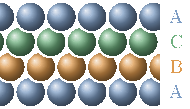
\includegraphics{fig01}

\vspace{0.4em}
{\scriptsize\color{cMuted} Вид сбоку: слои плотно упакованных шаров,\\ каждый следующий лежит в лунках предыдущего.}
\end{column}
\end{columns}

\vspace{0.6em}
{\footnotesize \statusProved{}\; Томас Хейлс (1998, с~С.~Фергюсоном); формальная машинная проверка — проект \emph{Flyspeck}, 2014.}
\end{frame}


\begin{frame}{Стадия 1: слой $A$ — плотнейшая укладка на плоскости}
\begin{columns}[T,onlytextwidth]
\begin{column}{0.50\textwidth}
\centering
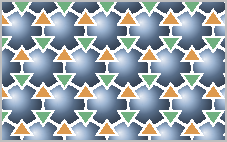
\includegraphics{fig02}

\vspace{0.35em}
{\scriptsize\color{cMuted} \textcolor{cLayB!80!black}{$\blacktriangle$} — лунки типа $B$\quad
\textcolor{cLayC!80!black}{$\blacktriangledown$} — лунки типа $C$}
\end{column}
\begin{column}{0.46\textwidth}
\vspace{0.4em}
\small
\begin{itemize}\itemsep3pt
  \item Каждый шар касается \textbf{шести} соседей: центры образуют треугольную решётку.
  \item Заполнение плоскости: $\pi/\sqrt{12} = 0.9069\ldots$
  \item Между шарами остаются лунки \textbf{двух} типов, отмеченные точками: $B$ (вершиной вверх) и $C$ (вершиной вниз).
  \item Лунок вдвое больше, чем шаров, но занять можно только половину — соседние лунки слишком близки.
\end{itemize}
\end{column}
\end{columns}
\end{frame}


\begin{frame}{Стадия 2: слой $B$ ложится в лунки}
\begin{columns}[T,onlytextwidth]
\begin{column}{0.50\textwidth}
\centering
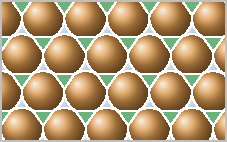
\includegraphics{fig03}

\vspace{0.35em}
{\scriptsize\color{cMuted} бледные — слой $A$, насыщенные — слой $B$,\\
\textcolor{cLayC!80!black}{$\blacktriangledown$} — оставшиеся свободными лунки $C$}
\end{column}
\begin{column}{0.46\textwidth}
\vspace{0.4em}
\small
\begin{itemize}\itemsep3pt
  \item Второй слой (оранжевый) занимает лунки типа $B$; выбор $B$ или $C$ здесь безразличен — конфигурации зеркальны.
  \item Расстояние между слоями: $h = 2R\sqrt{2/3} = 0.8165\cdot 2R$.
  \item Каждый шар слоя $B$ касается трёх шаров снизу; шар слоя $A$ — трёх шаров сверху.
  \item Свободными остаются лунки типа $C$ (зелёные точки) — именно они порождают развилку на следующем шаге.
\end{itemize}
\end{column}
\end{columns}
\end{frame}


\begin{frame}{Стадия 3: развилка — $ABAB\ldots$ или $ABCABC\ldots$}
\begin{columns}[T,onlytextwidth]
\begin{column}{0.48\textwidth}
\centering
{\small\textbf{Вариант 1: над $A$} $\;\Rightarrow\; ABAB\ldots$}\\[3pt]
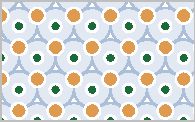
\includegraphics{fig04}

\vspace{2pt}
{\scriptsize\color{cMuted} Зелёные точки попадают в центры кругов $A$:\\ третий слой повторяет первый. \textbf{ГПУ} (\emph{hcp}).}
\end{column}
\begin{column}{0.48\textwidth}
\centering
{\small\textbf{Вариант 2: над $C$} $\;\Rightarrow\; ABCABC\ldots$}\\[3pt]
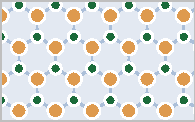
\includegraphics{fig05}

\vspace{2pt}
{\scriptsize\color{cMuted} Зелёные точки — в свободных лунках $C$:\\ появляется третье положение. \textbf{ГЦК} (\emph{fcc}).}
\end{column}
\end{columns}

\vspace{0.3em}
\centering
{\scriptsize\color{cMuted} круги — слой $A$\quad
\textcolor{cLayB!80!black}{$\bullet$}~слой $B$\quad
\textcolor{cProved}{$\bullet$}~третий слой}

\vspace{0.5em}
\raggedright
{\footnotesize Выбор независим на каждом шаге, поэтому плотнейших упаковок \textbf{континуум}: любая последовательность букв без двух одинаковых подряд даёт плотность $\pi/\sqrt{18}$.}
\end{frame}


\begin{frame}{Две регулярные укладки: числа}
\centering
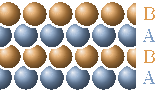
\includegraphics{fig06}
\hspace{1.2em}
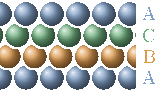
\includegraphics{fig07}

\vspace{0.2em}
{\scriptsize\color{cMuted} слева — $ABAB\ldots$ (ГПУ)\hspace{4.5em} справа — $ABCABC\ldots$ (ГЦК)}

\vspace{0.8em}
\footnotesize
\begin{tabular}{@{}lll@{}}
\toprule
 & ГПУ (\emph{hcp}) & ГЦК (\emph{fcc}) \\
\midrule
Последовательность слоёв & $ABAB\ldots$ & $ABCABC\ldots$ \\
Плотность & \multicolumn{2}{c}{$\pi/\sqrt{18} = 0.7404804\ldots$ (74.05\%)} \\
Доля пустот & \multicolumn{2}{c}{$25.95\%$} \\
Координационное число & \multicolumn{2}{c}{12 (6 в слое $+$ 3 сверху $+$ 3 снизу)} \\
Решётка Браве & не решётка (базис из 2 атомов) & гранецентрированная кубическая \\
Параметры & $c/a = \sqrt{8/3} = 1.633$ & $a = 2R\sqrt{2} = 2.828\,R$ \\
Пустоты на шар & \multicolumn{2}{c}{1 октаэдрическая $+$ 2 тетраэдрические} \\
\bottomrule
\end{tabular}
\end{frame}


\begin{frame}{Кристаллическая структура: ГЦК-ячейка меди}
\begin{columns}[T,onlytextwidth]
\begin{column}{0.46\textwidth}
\centering
\vspace{0.3em}
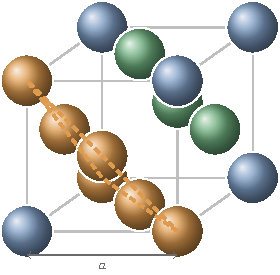
\includegraphics{fig08}

\vspace{0.4em}
{\scriptsize\color{cMuted}
\textcolor{cLayB!80!black}{$\bullet$}~6 атомов плоскости $(111)$\quad
\textcolor{cLayA!80!black}{$\bullet$}~вершины куба\quad
\textcolor{cLayC!80!black}{$\bullet$}~прочие центры граней\\[3pt]
Плоскость $(111)$ (оранжевый треугольник) — это и есть плотно упакованный слой $A$;\\
стопка таких плоскостей вдоль диагонали куба даёт $ABCABC\ldots$}
\end{column}
\begin{column}{0.50\textwidth}
\vspace{0.5em}
\footnotesize
\begin{tabular}{@{}ll@{}}
\toprule
Структурный тип & $A1$ (Cu), $Fm\bar{3}m$ \\
Атомов в ячейке & $8\cdot(1/8) + 6\cdot(1/2) = 4$ \\
Ребро ячейки & $a = 2R\sqrt{2}$ \\
Параметр меди & $a = 3.615$~\AA \\
Радиус атома Cu & $R = a/(2\sqrt2) = 1.278$~\AA \\
Координационное число & 12 \\
Плотность упаковки & $0.7405$ \\
\bottomrule
\end{tabular}

\vspace{0.8em}
{\footnotesize\raggedright Так же уложены Al, Ni, Ag, Au, Pt, Pb, $\gamma$-Fe и твёрдый Ar.
По типу ГПУ — Mg, Zn, Ti, Co, Cd.\par}
\end{column}
\end{columns}
\end{frame}


\begin{frame}{От шаров к квадратам}
\small
\begin{itemize}\itemsep4pt
  \item Для шаров в $\mathbb{R}^3$ задача \emph{решена}: оптимум известен и доказан, хотя оптимальных конфигураций бесконечно много.
  \item Для конечного числа квадратов в квадрате картина обратная: конструкции выглядят хаотично, а доказательства оптимальности есть лишь для небольших $n$.
  \item Общего принципа нет: оптимум не обязан быть симметричным и не обязан состоять из одинаково ориентированных элементов.
\end{itemize}
\vspace{0.8em}
\centering
{\footnotesize Дальше — таблица известных результатов для упаковки $n$ единичных квадратов.}
\end{frame}


\section*{}
\begin{frame}[plain]
\vfill
\centering
{\Large\bfseries Часть II. Упаковка единичных квадратов в квадрат}\\[6pt]
{\color{cMuted}\small числовые данные и статус доказанности}
\vfill
\end{frame}

\begin{frame}{Как читать слайды}
\footnotesize
\begin{itemize}
  \item $n$ — число единичных квадратов; $s$ — сторона внешнего квадрата.
  \item Запись вида $s = 4.675{+}$ означает \emph{«чуть больше»}: приведено округление снизу, а не точное равенство.
  \item Плотность заполнения: $\rho = n / s^2$ — доля площади контейнера, занятая квадратами.
  \item Статусы:
  \begin{itemize}
    \item \statusProved{} — на странице явно указано \emph{Proved by}: минимальность стороны доказана.
    \item \statusFound{} — указано \emph{Found by}: это верхняя оценка $s_n \le \ldots$; оптимальность \textbf{не} доказана.
    \item \statusTrivial{} — очевидная раскладка без наклонённых квадратов.
  \end{itemize}
  \item Иллюстрации для $n \le 11$, $14$, $15$, $17\ldots19$ и $52\ldots55$ — оригинальные схемы
        Эриха Фридмана; для $n = 12, 13, 16, 20$ тривиальные раскладки построены в TikZ.
  \item Серый квадрат — единичный; тонкая рамка — контейнер со стороной $s$.
\end{itemize}
\end{frame}

\begin{frame}{Сводка}
\footnotesize
\centering
\begin{tabular}{@{}lr p{0.46\textwidth}@{}}
\toprule
Статус & Случаев & Значения $n$ \\
\midrule

\statusTrivial & 4 & 1, 4, 9, 16 \\
\statusTrivBest & 3 & 12, 13, 20 \\
\statusProved & 9 & 2, 3, 5, 6, 7, 8, 10, 14, 15 \\
\statusFound & 8 & \raggedright\arraybackslash 11, 17, 18, 19, 52, 53, 54, 55 \\
\bottomrule
\end{tabular}

\vspace{1em}
\begin{minipage}{0.86\textwidth}\scriptsize\color{cMuted}
Показаны все $n \le 20$, а также блок $n = 52\ldots55$. Для $n = 12, 13, 16, 20$ страница
иллюстраций не даёт: там лучшей известной остаётся тривиальная раскладка без наклонённых квадратов.
Доказательства оптимальности известны лишь для малых $n$; остальные записи — рекордные конструкции.
\end{minipage}
\end{frame}


\begin{frame}{Упаковки $n = 1\ldots4$}
\centering
\vspace{0.4em}

\begin{minipage}[t]{0.48\textwidth}
\begin{minipage}[c]{2.8cm}
\imgphs{2.7}{1}
\end{minipage}%
\hfill
\begin{minipage}[c]{2.9cm}
\raggedright
{\scriptsize $n = 1$}\\[1pt]
{\scriptsize $s = 1$}\\[1pt]
{\scriptsize $n/s^2 = 1.000$}\\[3pt]
{\scriptsize \statusTrivial}
\end{minipage}
\end{minipage}
\hfill
\begin{minipage}[t]{0.48\textwidth}
\begin{minipage}[c]{2.8cm}
\imgphs{2.7}{2}
\end{minipage}%
\hfill
\begin{minipage}[c]{2.9cm}
\raggedright
{\scriptsize $n = 2$}\\[1pt]
{\scriptsize $s = 2$}\\[1pt]
{\scriptsize $n/s^2 = 0.500$}\\[3pt]
{\scriptsize \statusProved}\\[1pt]
{\scriptsize\color{cMuted} Frits Göbel, 1979}
\end{minipage}
\end{minipage}

\vspace{1.2em}

\begin{minipage}[t]{0.48\textwidth}
\begin{minipage}[c]{2.8cm}
\imgphs{2.7}{3}
\end{minipage}%
\hfill
\begin{minipage}[c]{2.9cm}
\raggedright
{\scriptsize $n = 3$}\\[1pt]
{\scriptsize $s = 2$}\\[1pt]
{\scriptsize $n/s^2 = 0.750$}\\[3pt]
{\scriptsize \statusProved}\\[1pt]
{\scriptsize\color{cMuted} Frits Göbel, 1979}
\end{minipage}
\end{minipage}
\hfill
\begin{minipage}[t]{0.48\textwidth}
\begin{minipage}[c]{2.8cm}
\imgphs{2.7}{4}
\end{minipage}%
\hfill
\begin{minipage}[c]{2.9cm}
\raggedright
{\scriptsize $n = 4$}\\[1pt]
{\scriptsize $s = 2$}\\[1pt]
{\scriptsize $n/s^2 = 1.000$}\\[3pt]
{\scriptsize \statusTrivial}
\end{minipage}
\end{minipage}

\vspace{1.2em}

\end{frame}


\begin{frame}{Упаковки $n = 5\ldots8$}
\centering
\vspace{0.4em}

\begin{minipage}[t]{0.48\textwidth}
\begin{minipage}[c]{2.8cm}
\imgphs{2.7}{5}
\end{minipage}%
\hfill
\begin{minipage}[c]{2.9cm}
\raggedright
{\scriptsize $n = 5$}\\[1pt]
{\scriptsize $s = 2 + \tfrac{1}{\sqrt{2}} = 2.707{+}$}\\[1pt]
{\scriptsize $n/s^2 = 0.682$}\\[3pt]
{\scriptsize \statusProved}\\[1pt]
{\scriptsize\color{cMuted} Frits Göbel, 1979}
\end{minipage}
\end{minipage}
\hfill
\begin{minipage}[t]{0.48\textwidth}
\begin{minipage}[c]{2.8cm}
\imgphs{2.7}{6}
\end{minipage}%
\hfill
\begin{minipage}[c]{2.9cm}
\raggedright
{\scriptsize $n = 6$}\\[1pt]
{\scriptsize $s = 3$}\\[1pt]
{\scriptsize $n/s^2 = 0.667$}\\[3pt]
{\scriptsize \statusProved}\\[1pt]
{\scriptsize\color{cMuted} Michael Kearney, Peter Shiu, апрель 2002}
\end{minipage}
\end{minipage}

\vspace{1.2em}

\begin{minipage}[t]{0.48\textwidth}
\begin{minipage}[c]{2.8cm}
\imgphs{2.7}{7}
\end{minipage}%
\hfill
\begin{minipage}[c]{2.9cm}
\raggedright
{\scriptsize $n = 7$}\\[1pt]
{\scriptsize $s = 3$}\\[1pt]
{\scriptsize $n/s^2 = 0.778$}\\[3pt]
{\scriptsize \statusProved}\\[1pt]
{\scriptsize\color{cMuted} Erich Friedman, 1999}
\end{minipage}
\end{minipage}
\hfill
\begin{minipage}[t]{0.48\textwidth}
\begin{minipage}[c]{2.8cm}
\imgphs{2.7}{8}
\end{minipage}%
\hfill
\begin{minipage}[c]{2.9cm}
\raggedright
{\scriptsize $n = 8$}\\[1pt]
{\scriptsize $s = 3$}\\[1pt]
{\scriptsize $n/s^2 = 0.889$}\\[3pt]
{\scriptsize \statusProved}\\[1pt]
{\scriptsize\color{cMuted} Erich Friedman, 1999}
\end{minipage}
\end{minipage}

\vspace{1.2em}

\end{frame}


\begin{frame}{Упаковки $n = 9\ldots12$}
\centering
\vspace{0.4em}

\begin{minipage}[t]{0.48\textwidth}
\begin{minipage}[c]{2.8cm}
\imgphs{2.7}{9}
\end{minipage}%
\hfill
\begin{minipage}[c]{2.9cm}
\raggedright
{\scriptsize $n = 9$}\\[1pt]
{\scriptsize $s = 3$}\\[1pt]
{\scriptsize $n/s^2 = 1.000$}\\[3pt]
{\scriptsize \statusTrivial}
\end{minipage}
\end{minipage}
\hfill
\begin{minipage}[t]{0.48\textwidth}
\begin{minipage}[c]{2.8cm}
\imgphs{2.7}{10}
\end{minipage}%
\hfill
\begin{minipage}[c]{2.9cm}
\raggedright
{\scriptsize $n = 10$}\\[1pt]
{\scriptsize $s = 3 + \tfrac{1}{\sqrt{2}} = 3.707{+}$}\\[1pt]
{\scriptsize $n/s^2 = 0.728$}\\[3pt]
{\scriptsize \statusProved}\\[1pt]
{\scriptsize\color{cMuted} Walter Stromquist, 2003}
\end{minipage}
\end{minipage}

\vspace{1.2em}

\begin{minipage}[t]{0.48\textwidth}
\begin{minipage}[c]{2.8cm}
\imgphs{2.7}{11}
\end{minipage}%
\hfill
\begin{minipage}[c]{2.9cm}
\raggedright
{\scriptsize $n = 11$}\\[1pt]
{\scriptsize $s = 3.877{+}$}\\[1pt]
{\scriptsize $n/s^2 = 0.732$}\\[3pt]
{\scriptsize \statusFound}\\[1pt]
{\scriptsize\color{cMuted} Walter Trump, 1979}
\end{minipage}
\end{minipage}
\hfill
\begin{minipage}[t]{0.48\textwidth}
\begin{minipage}[c]{2.8cm}
\imgphs{2.7}{12}
\end{minipage}%
\hfill
\begin{minipage}[c]{2.9cm}
\raggedright
{\scriptsize $n = 12$}\\[1pt]
{\scriptsize $s = 4$}\\[1pt]
{\scriptsize $n/s^2 = 0.750$}\\[3pt]
{\scriptsize \statusTrivBest}
\end{minipage}
\end{minipage}

\vspace{1.2em}

\end{frame}


\begin{frame}{Упаковки $n = 13\ldots16$}
\centering
\vspace{0.4em}

\begin{minipage}[t]{0.48\textwidth}
\begin{minipage}[c]{2.8cm}
\imgphs{2.7}{13}
\end{minipage}%
\hfill
\begin{minipage}[c]{2.9cm}
\raggedright
{\scriptsize $n = 13$}\\[1pt]
{\scriptsize $s = 4$}\\[1pt]
{\scriptsize $n/s^2 = 0.812$}\\[3pt]
{\scriptsize \statusTrivBest}
\end{minipage}
\end{minipage}
\hfill
\begin{minipage}[t]{0.48\textwidth}
\begin{minipage}[c]{2.8cm}
\imgphs{2.7}{14}
\end{minipage}%
\hfill
\begin{minipage}[c]{2.9cm}
\raggedright
{\scriptsize $n = 14$}\\[1pt]
{\scriptsize $s = 4$}\\[1pt]
{\scriptsize $n/s^2 = 0.875$}\\[3pt]
{\scriptsize \statusProved}\\[1pt]
{\scriptsize\color{cMuted} Erich Friedman, 1999}
\end{minipage}
\end{minipage}

\vspace{1.2em}

\begin{minipage}[t]{0.48\textwidth}
\begin{minipage}[c]{2.8cm}
\imgphs{2.7}{15}
\end{minipage}%
\hfill
\begin{minipage}[c]{2.9cm}
\raggedright
{\scriptsize $n = 15$}\\[1pt]
{\scriptsize $s = 4$}\\[1pt]
{\scriptsize $n/s^2 = 0.938$}\\[3pt]
{\scriptsize \statusProved}\\[1pt]
{\scriptsize\color{cMuted} Erich Friedman, 1999}
\end{minipage}
\end{minipage}
\hfill
\begin{minipage}[t]{0.48\textwidth}
\begin{minipage}[c]{2.8cm}
\imgphs{2.7}{16}
\end{minipage}%
\hfill
\begin{minipage}[c]{2.9cm}
\raggedright
{\scriptsize $n = 16$}\\[1pt]
{\scriptsize $s = 4$}\\[1pt]
{\scriptsize $n/s^2 = 1.000$}\\[3pt]
{\scriptsize \statusTrivial}
\end{minipage}
\end{minipage}

\vspace{1.2em}

\end{frame}


\begin{frame}{Упаковки $n = 17\ldots20$}
\centering
\vspace{0.4em}

\begin{minipage}[t]{0.48\textwidth}
\begin{minipage}[c]{2.8cm}
\imgphs{2.7}{17}
\end{minipage}%
\hfill
\begin{minipage}[c]{2.9cm}
\raggedright
{\scriptsize $n = 17$}\\[1pt]
{\scriptsize $s = 4.675{+}$}\\[1pt]
{\scriptsize $n/s^2 = 0.778$}\\[3pt]
{\scriptsize \statusFound}\\[1pt]
{\scriptsize\color{cMuted} John Bidwell, 1997}
\end{minipage}
\end{minipage}
\hfill
\begin{minipage}[t]{0.48\textwidth}
\begin{minipage}[c]{2.8cm}
\imgphs{2.7}{18}
\end{minipage}%
\hfill
\begin{minipage}[c]{2.9cm}
\raggedright
{\scriptsize $n = 18$}\\[1pt]
{\scriptsize $s = \tfrac{7 + \sqrt{7}}{2} = 4.822{+}$}\\[1pt]
{\scriptsize $n/s^2 = 0.774$}\\[3pt]
{\scriptsize \statusFound}\\[1pt]
{\scriptsize\color{cMuted} Pertti Hämäläinen, 1979}
\end{minipage}
\end{minipage}

\vspace{1.2em}

\begin{minipage}[t]{0.48\textwidth}
\begin{minipage}[c]{2.8cm}
\imgphs{2.7}{19}
\end{minipage}%
\hfill
\begin{minipage}[c]{2.9cm}
\raggedright
{\scriptsize $n = 19$}\\[1pt]
{\scriptsize $s = 3 + 4\sqrt{2}/3 = 4.885{+}$}\\[1pt]
{\scriptsize $n/s^2 = 0.796$}\\[3pt]
{\scriptsize \statusFound}\\[1pt]
{\scriptsize\color{cMuted} Robert Wainwright, 1979}
\end{minipage}
\end{minipage}
\hfill
\begin{minipage}[t]{0.48\textwidth}
\begin{minipage}[c]{2.8cm}
\imgphs{2.7}{20}
\end{minipage}%
\hfill
\begin{minipage}[c]{2.9cm}
\raggedright
{\scriptsize $n = 20$}\\[1pt]
{\scriptsize $s = 5$}\\[1pt]
{\scriptsize $n/s^2 = 0.800$}\\[3pt]
{\scriptsize \statusTrivBest}
\end{minipage}
\end{minipage}

\vspace{1.2em}

\end{frame}


\begin{frame}{$n = 17$: симметричная упаковка и упаковка Бидвелла}
\centering

\begin{minipage}[b]{4.6cm}
\centering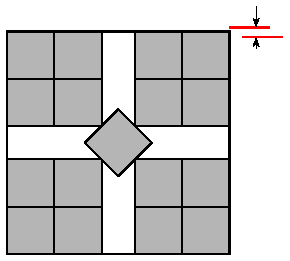
\includegraphics{cmp17}
\end{minipage}%
\hspace{0.4cm}%
\begin{minipage}[b]{4.1cm}
\centering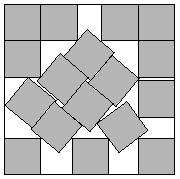
\includegraphics[width=3.9604cm]{17}
\end{minipage}

\vspace{0.35em}

{\footnotesize
\begin{tabular}{@{}l c c@{}}
\toprule
 & симметричная & Бидвелл, 1997 \\
\midrule
Сторона $s$ & $4 + \tfrac{1}{\sqrt{2}} = 4.70711$ & $4.67553\ldots$ \\
Площадь $s^2$ & $22.15685$ & $21.86058$ \\
Плотность $\rho = 17/s^2$ & $0.76726$ & $0.77766$ \\
Ориентаций квадратов & $2$ ($0^\circ$, $45^\circ$) & $3$ \\
Поворотная симметрия & $90^\circ$ & нет \\
$\Delta s$ & $+0.03158$ ($+0.68\%$) & — \\
\bottomrule
\end{tabular}}
\end{frame}


\begin{frame}{Упаковки $n = 52\ldots55$}
\centering
\vspace{0.4em}

\begin{minipage}[t]{0.48\textwidth}
\begin{minipage}[c]{2.8cm}
\imgphs{2.7}{52}
\end{minipage}%
\hfill
\begin{minipage}[c]{2.9cm}
\raggedright
{\scriptsize $n = 52$}\\[1pt]
{\scriptsize $s = 7 + \tfrac{1}{\sqrt{2}} = 7.707{+}$}\\[1pt]
{\scriptsize $n/s^2 = 0.875$}\\[3pt]
{\scriptsize \statusFound}\\[1pt]
{\scriptsize\color{cMuted} Frits Göbel, 1979}
\end{minipage}
\end{minipage}
\hfill
\begin{minipage}[t]{0.48\textwidth}
\begin{minipage}[c]{2.8cm}
\imgphs{2.7}{53}
\end{minipage}%
\hfill
\begin{minipage}[c]{2.9cm}
\raggedright
{\scriptsize $n = 53$}\\[1pt]
{\scriptsize $s = 7.823{+}$}\\[1pt]
{\scriptsize $n/s^2 = 0.866$}\\[3pt]
{\scriptsize \statusFound}\\[1pt]
{\scriptsize\color{cMuted} David W. Cantrell, сентябрь 2002}
\end{minipage}
\end{minipage}

\vspace{1.2em}

\begin{minipage}[t]{0.48\textwidth}
\begin{minipage}[c]{2.8cm}
\imgphs{2.7}{54}
\end{minipage}%
\hfill
\begin{minipage}[c]{2.9cm}
\raggedright
{\scriptsize $n = 54$}\\[1pt]
{\scriptsize $s = 7.846{+}$}\\[1pt]
{\scriptsize $n/s^2 = 0.877$}\\[3pt]
{\scriptsize \statusFound}\\[1pt]
{\scriptsize\color{cMuted} Joe DeVincentis, апрель 2014}
\end{minipage}
\end{minipage}
\hfill
\begin{minipage}[t]{0.48\textwidth}
\begin{minipage}[c]{2.8cm}
\imgphs{2.7}{55}
\end{minipage}%
\hfill
\begin{minipage}[c]{2.9cm}
\raggedright
{\scriptsize $n = 55$}\\[1pt]
{\scriptsize $s = 7.954{+}$}\\[1pt]
{\scriptsize $n/s^2 = 0.869$}\\[3pt]
{\scriptsize \statusFound}\\[1pt]
{\scriptsize\color{cMuted} Joe DeVincentis, апрель 2014}
\end{minipage}
\end{minipage}

\vspace{1.2em}

\end{frame}


\begin{frame}{Итог}
\small
\begin{itemize}
  \item Доказанная оптимальность известна лишь для небольших $n$; для остальных приведены
        рекордные конструкции, и знак «+» подчёркивает, что это верхняя оценка.
  \item Наиболее известный пример — $n = 17$, $s = 4.675{+}$ (John Bidwell, 1997).
  \item Формулировка «optimal packing», распространённая в интернете, для большинства $n$
        некорректна: речь о \emph{наименьшем известном} квадрате.
\end{itemize}
\vspace{0.8em}
{\scriptsize\color{cMuted} Источник: Erich Friedman, \emph{Squares in Squares} —
\texttt{https://tabatkins.github.io/efmath/packing/squinsqu/}\\
См. также: Erich Friedman, \emph{Packing Unit Squares in Squares: A Survey and New Results},
Electronic Journal of Combinatorics, DS7.}
\end{frame}

\end{document}
